Use Root-Locus analysis to answer the questions about the following feedback control system.

\begin{center}
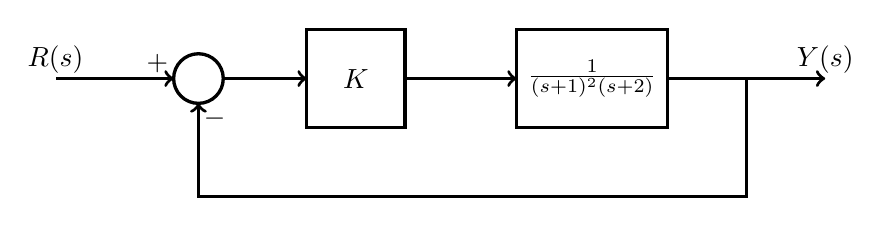
\begin{tikzpicture}[scale=1,inner sep=0pt,outer sep=0pt,very thick,
sysblock/.style={draw,rectangle,inner sep=4pt,minimum width=1.25cm,minimum height=1.25cm,very thick}]

\draw (-2,0) node[draw,circle] (sum1) {$\rule{0pt}{18pt}$};
\draw (0,0) node[sysblock] (K)  {$K$};
\draw (3,0) node[sysblock] (G) {$\frac{1}{(s+1)^2(s+2)}$};
\draw[<-] (sum1.180) node[above left=2pt] {$+$} -- ++(-1.5,0) node[above=2pt] {$R(s)$};
\draw[->] (sum1.0) -- (K.180);
\draw[->] (K.0) -- (G.180);
\draw[->] (G.0) --  ++(2,0) node[above=2pt] {$Y(s)$};
\draw[->] (G.0) -- ++(1,0) -- ++(0,-1.5) -| (sum1.-90) node[below right=2pt] {$-$};
\end{tikzpicture}
\end{center}

\begin{enumerate}[(a)]
\item Sketch the root locus for this system. You can use the plotting rules we learned in class or Matlab.
\item Find the point on the imaginary axis where the poles cross over from the left-half to the right-half plane. \textit{Hint 1: closed-loop poles are values of $s$ that satisfy $1+KG(s)=0$. Hint 2: a pole on the imaginary axis -- i.e., at the stability boundary -- will have a value of $s=j\omega$, i.e., real part equal to zero. Hint 3: to make a complex equation equal to zero, both real and imaginary parts must equal 0.} 
\item Find the value $K$ that corresponds to the crossing point found in part (b). \textit{Hint: use one of the equations you found in part (b) containing both $K$ and $\omega$.}
\end{enumerate}
